\subsection{Temporal \& Spatial Aggregation Model}
\frame{\frametitle{Outline}\tableofcontents[currentsection,currentsubsection]}


\frame
{
   \frametitle{Temporal \& Spatial Aggregation Model}
   \begin{itemize}
   \item Enable large-scale trace analysis
   \item Visualy compare entities behavior
   \item Detect global and local characteristics

   \vfill

   \begin{block}{Steps of the Model}
      \begin{enumerate}
      \item Hierarchical Monitoring Data
      \item Temporal Aggregation
      \item Spatial Aggregation
      \item Treemap representation
      \end{enumerate}
   \end{block}

%   \vfill
%   \item Differences from existing tools
%      \begin{itemize}
%      \item PlanetLab's CoVisualize $\rightarrow$ resources
%      \item Treemap for Workload Visualization [Stephen 2003]
%      \vspace{.2cm}
%      \item Lack of configurable time intervals
%      \end{itemize}
   \end{itemize}
}

%\frame
%{
%   \frametitle{Hierarchical Monitoring Data}
%   \begin{itemize}
%      \item Monitoring systems register entities behavior
%      \item Entities can be processes and threads
%      \item They can be organized as a hierarchy
%	 \begin{itemize}
%	    \item Logical hierarchy
%	    \item Geographical Location hierarchy
%	    \item Other possibilities: libraries, components
%	 \end{itemize}
%      \item Grid'5000 example
%   \end{itemize}
%
%   \vfill
%
%   \begin{minipage}{\textwidth}
%   \centering
%   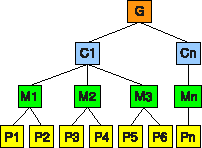
\includegraphics[width=.5\textwidth]{img/hierarchical-mon-data-4.pdf}
%   \end{minipage}
%}
%

\frame
{
   \frametitle{Temporal Aggregation - Basics}
   \begin{block}{Objective: annotate leaves of the hierarchy}
      \begin{itemize}
      \item Time-slice definition
      \item Summary of trace events on the interval
	 \begin{itemize}
	 \item States, Variables, Links, Events, ...
	 \end{itemize}
      \end{itemize}
   \end{block}

   \vfill

%   \begin{block}{Output of the Algorithm}
%      \begin{itemize}
%      \item Hierarchy of input
%      \item Computed values on leaves
%      \end{itemize}
%   \end{block}
%
%   \vfill

   \hspace{-.7cm}
   \begin{minipage}{\textwidth}
   \centering
   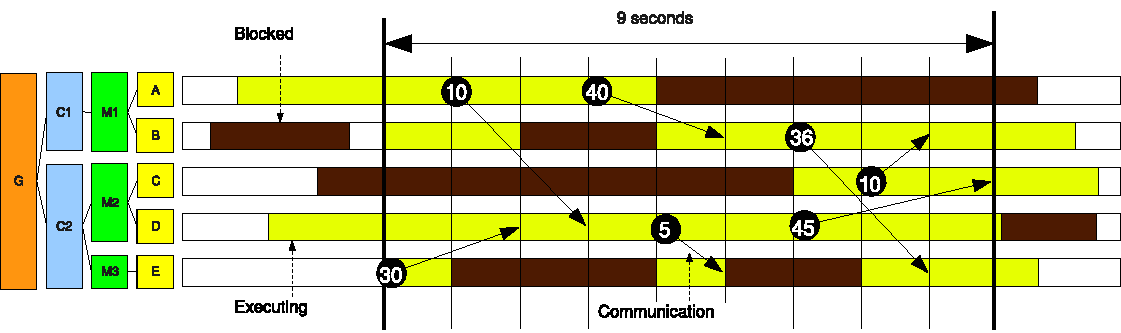
\includegraphics[width=1.1\textwidth]{img/agg-ts-complete-example.pdf}
   \end{minipage}
}

\frame
{
   \frametitle{Temporal Aggregation - Example}

   \hspace{-.7cm}
   \begin{minipage}{\textwidth}
   \centering
   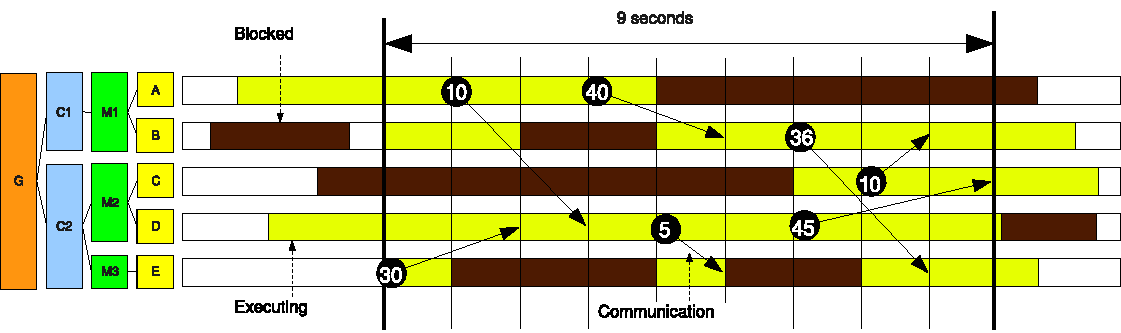
\includegraphics[width=1.1\textwidth]{img/agg-ts-complete-example.pdf}
   \end{minipage}

   \vfill

   \begin{minipage}{\textwidth}
   \centering
   \includegraphics[width=.6\textwidth]<1>
      {img/agg-ts-complete-example-hierarchy.pdf}
   \includegraphics[width=.5\textwidth]<2>
      {img/agg-ts-complete-example-hierarchy-merged-new.pdf}
   \end{minipage}
   
   \vfill
}



\frame
{
   \frametitle{Spatial Aggregation}

   \begin{itemize}
   \item Explore the hierarchical organization
   \item Create aggregated values at intermediary levels
   \end{itemize}

   \begin{block}{Aggregation Functions}
      \begin{itemize}
      \item add, subtract, multiply, divide, max, min, median, ...
      \item Depends on
	 \begin{itemize}
	 \item what type of value the leaves have
	 \item the desired statistical result
	 \end{itemize}
      \end{itemize}
   \end{block}

   \vfill

   \begin{minipage}{\textwidth}
   \centering
   \includegraphics[width=.6\textwidth]<1>{img/agg-aggmodel-overall-1.pdf}
   \includegraphics[width=.6\textwidth]<2>{img/agg-aggmodel-overall-2.pdf}
   \includegraphics[width=.6\textwidth]<3>{img/agg-aggmodel-overall-3.pdf}
   \includegraphics[width=.6\textwidth]<4>{img/agg-aggmodel-overall-4.pdf}
   \end{minipage}
}

\frame
{
   \frametitle{Visualization of the Approach - Treemaps}
   \begin{itemize}
      \item Scalable hierarchical representation
      \item Top-down drawing algorithm
      \item For a given node, split screen space among children
   \end{itemize}

   \vfill

   \begin{minipage}{\textwidth}
   \centering
   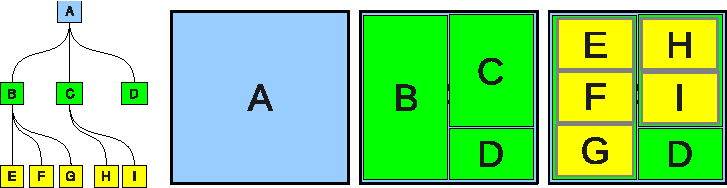
\includegraphics[width=\textwidth]{img/treemap-notion.pdf}
   \end{minipage}

   \vfill

   \begin{block}{Original algorithm has several evolutions}
   \begin{itemize}
      \item Squarified treemap is used here
      \item Keeps rectangles as close to squares as possible
   \end{itemize}
   \end{block}
}

\frame
{
   \frametitle{Treemap to view the Aggregated Hierarchy}

   \begin{minipage}{\textwidth}
   \centering
   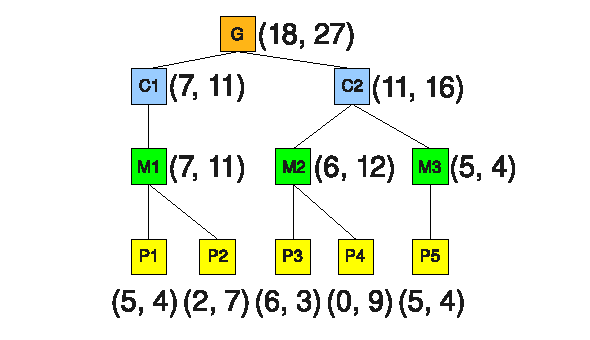
\includegraphics[width=.7\textwidth]{img/agg-aggmodel-overall-4.pdf}\\
   \includegraphics<1>[width=.28\textwidth]{img/agg-aggmodel-treemap-1.pdf}
   \includegraphics<2>[width=.28\textwidth]{img/agg-aggmodel-treemap-2.pdf}
   \includegraphics<3>[width=.28\textwidth]{img/agg-aggmodel-treemap-3.pdf}
   \includegraphics<4>[width=.28\textwidth]{img/agg-aggmodel-treemap-4.pdf}
   \end{minipage}
}
